\documentclass[tikz]{standalone}

\usepackage{tikz}
\usetikzlibrary{arrows.meta,
                positioning,
                quotes}
\usepackage{mathtools,nccmath}
\tikzstyle{fleche}=[->,>=stealth,thick,rounded corners=4pt]
%Sparse matrices
\def\ArrPlus{%
\setbox0\hbox{$\longleftrightarrow$}%
\rlap{\hbox to \wd0{\hss\rotatebox[origin=top]{90}{\scalebox{.9}{$\longleftrightarrow$}}\hss}}\raise.15ex\box0}
\def\arrowplus{\mathbin{%
\mathchoice
  {\scalebox{.7}{\ArrPlus}}
  {\scalebox{.7}{\ArrPlus}}
  {\scalebox{.35}{\raisebox{.2ex}{\ArrPlus}}}
  {\scalebox{.25}{\raisebox{.35ex}{\ArrPlus}}}
}}

\newcommand*\markterm[2]{%
	\tikz[remember picture,anchor=base west,baseline,inner sep=0pt, outer sep=0pt]\node(#1){$#2$};%
}
\newcommand*\arrowtoterm[3][]{%
	\tikz[remember picture,anchor=base west,baseline,inner sep=0pt, outer sep=0pt]\node(x){#3};%
	\tikz[remember picture,overlay,->,shorten <=2pt,shorten >=2pt,#1]\draw(x)to(#2);%
}


\begin{document}

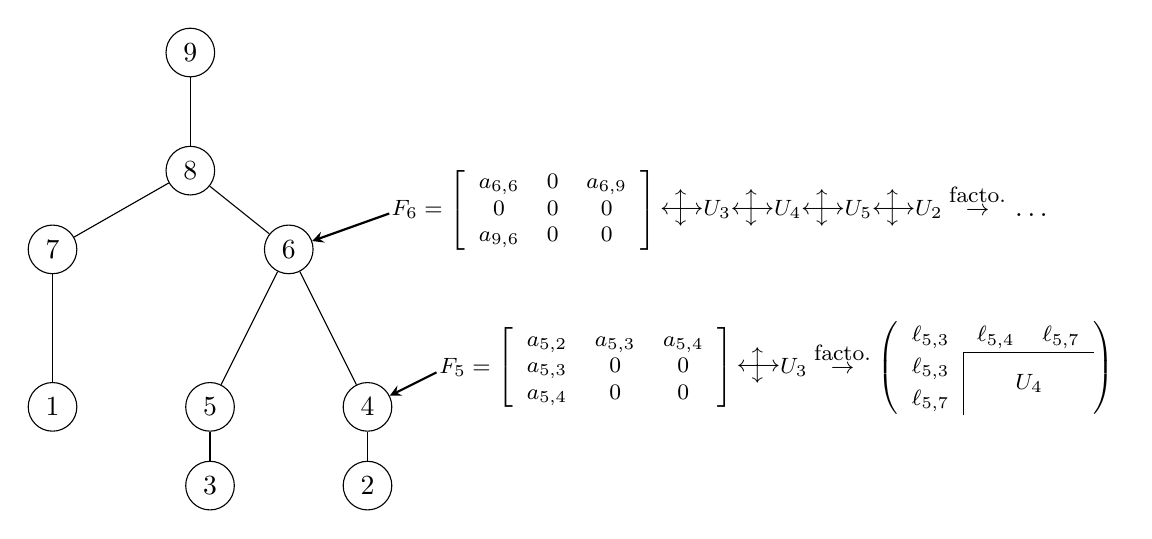
\begin{tikzpicture}
    \node[draw,circle] (1) at (-1,1) {1};
    \node[draw,circle] (3) at (1,0) {3};
    \node[draw,circle] (2) at (3,0) {2};
    \node[draw,circle] (5) at (1,1) {5};
    \node[draw,circle] (4) at (3,1) {4};
    \node[draw,circle] (6) at (2,3) {6};
    \node[draw,circle] (7) at (-1,3) {7};
    \node[draw,circle] (8) at (0.75,4) {8};
    \node[draw,circle] (9) at (0.75,5.5) {9};
    \draw (1) -- (7);
    \draw (7) -- (8);
    \draw (8) -- (9);
    \draw (6) -- (8);
    \draw (4) -- (6);
    \draw (5) -- (6);
    \draw (2) -- (4);
    \draw (3) -- (5);
    \node (F4) at (4,1.5) {};
    \node (F6) at (3.4,3.5) {};

    \node (eq) at (8.2,1.5) {$\medmath{F_5=\left[\begin{array}{ccc} a_{5,2} & a_{5,3} & a_{5,4} \\ a_{5,3} & 0 & 0 \\ a_{5,4} & 0 & 0 \end{array}\right] \ArrPlus U_3 \stackrel{\mbox{facto.}}{\rightarrow} 
  \renewcommand{\arraystretch}{1.2}
  \left(
  \begin{array}{  c c c }
    \ell_{5,3} & \ell_{5,4} & \ell_{5,7} \\
    \cline{2-3}
    \ell_{5,3} & \multicolumn{1}{|c}{} & \multicolumn{1}{c}{} \\
    \ell_{5,7} & \multicolumn{2}{|c}{\raisebox{.6\normalbaselineskip}[0pt][0pt]{$U_4$}} \\
    % \cline{2-3}
  \end{array}
  \right)
    }$};

    \node (eq) at (7.5,3.5) {$\medmath{F_6=\left[\begin{array}{ccc} a_{6,6} & 0 & a_{6,9} \\ 0 & 0 & 0 \\ a_{9,6} & 0 & 0 \end{array}\right] \ArrPlus U_3 \ArrPlus U_4 \ArrPlus U_5 \ArrPlus U_2 \stackrel{\mbox{facto.}}{\rightarrow}}$ \dots };
    \draw[fleche] (F4) -- (4);
    \draw[fleche] (F6) -- (6);


\end{tikzpicture}

\end{document}